\documentclass[a4paper,12pt,oneside]{book} % nie: report!


% pakiety
\usepackage{polski} % lepiej to zamiast babel!
\usepackage[utf8]{inputenc} % w razie kłopotów spróbować: \usepackage[utf8x]{inputenc}
\usepackage{fancyhdr} % nagłówki i stopki
\usepackage{indentfirst} % WAŻNE, MA BYĆ!
\usepackage[pdftex]{graphicx} % to do wstawiania rysunków
\usepackage{amsmath} % to do dodatkowych symboli, przydatne
\usepackage[pdftex,
            left=1in,right=1in,
            top=1in,bottom=1in]{geometry} % marginsy
\usepackage{amssymb} % to też do dodatkowych symboli, też przydatne
\usepackage{pdfpages}
\usepackage{lipsum}
\usepackage{multirow}
\usepackage{listings}
\usepackage{caption}
\usepackage{booktabs}
\usepackage{subcaption}
\usepackage{xcolor}
\usepackage{url}
\usepackage{tikz} 
\graphicspath{ {./grafika/} }
\DeclareCaptionType{code}[Listing][Spis listingów] 

\definecolor{codegreen}{rgb}{0,0.6,0}
\definecolor{codegray}{rgb}{0.5,0.5,0.5}
\definecolor{codepurple}{rgb}{0.58,0,0.82}
\definecolor{backcolour}{rgb}{0.95,0.95,0.92}

\def\crnrs#1{$^\ulcorner#1_\lrcorner$}
\lstset{
	backgroundcolor=\color{backcolour},   
	commentstyle=\color{codegreen},
	keywordstyle=\color{magenta},
	numberstyle=\tiny\color{codegray},
	stringstyle=\color{codepurple},
	basicstyle=\ttfamily\footnotesize,
	breakatwhitespace=false,         
	breaklines=true,                 
	captionpos=b,                    
	keepspaces=true,                 
	numbers=left,                    
	numbersep=5pt,                  
	showspaces=false,                
	showstringspaces=false,
	showtabs=false,                  
	tabsize=2,
	float=h
}

% definicje nagłówków i stopek
\pagestyle{fancy}
\renewcommand{\chaptermark}[1]{\markboth{#1}{}}
\renewcommand{\sectionmark}[1]{\markright{\thesection\ #1}}
\fancyhf{}
\fancyhead[LE,RO]{\footnotesize\bfseries\thepage}
\fancyhead[LO]{\footnotesize\rightmark}
\fancyhead[RE]{\footnotesize\leftmark}
\renewcommand{\headrulewidth}{0.5pt}
\renewcommand{\footrulewidth}{0pt}
\addtolength{\headheight}{1.5pt}
\fancypagestyle{plain}{\fancyhead{}\cfoot{\footnotesize\bfseries\thepage}\renewcommand{\headrulewidth}{0pt}}


% interlinia
\linespread{1.25}


% treść
\begin{document}
\sloppy
\thispagestyle{empty}
\includepdf{stronatytulowa}
\newpage{}

\thispagestyle{empty}
\newpage{}

\tableofcontents{}

\chapter*{Wstęp} 

Rośliny to rozległa grupa organizmów żywych, występujących na większości 
lądów na Ziemi, a także w środowisku wodnym. 
Należą do nich trawy, drzewa, kwiaty, krzewy, paprocie, mchy i wiele innych.
Istnieje około 391,000 gatunków roślin, z których zdecydowana większość,
około 369,000 (94\%), wytwarza nasiona.\cite{howmanyplants} Rośliny można znaleźć na 
całym świecie, na wszystkich kontynentach. Rośliny dostarczają znaczną część 
tlenu na świecie i stanowią podstawę
większości ekosystemów na Ziemi. Tak ważna część świata rzeczywistego prędzej 
czy później wymagała matematycznego opisu i dalszego zastosowania w różnych rodzajach nauki, w
szczególności w informatyce. Modelowanie roślin w informatyce
jest szeroko stosowane w wielu dziedzinach, takich jak gry, przemysł filmowy, 
agrokultura i architektura. Rośliny charakteryzują się złożoną,
zwykle fraktalną strukturą, która jest trudna do modelowania.
Z tego powodu opracowano różne systemy opisywania modeli roślin,
aby uporządkować i uprościć pracę z modelowaniem drzew. Jednym z
takich systemów jest system Lindenmaiera, który umożliwia opis struktur 
fraktalnych, w szczególności roślin na poziomie gramatyki formalnej.

\addcontentsline{toc}{chapter}{Wstęp}


% \chapter*{Cel pracy} 

Celem tej pracy jest analiza i zapoznanie się z systemem Lindenmayera, 
możliwościami jego rozbudowy i wykorzystania do generowania roślin, 
a konkretnie drzew. Ponadto należy opracować oprogramowanie umożliwiające 
tworzenie trójwymiarowych modeli drzew z możliwością modyfikacji 
parametrów drzew i symulacji ich wzrostu. Oprogramowanie powinno posiadać 
następujące funkcje:

\begin{itemize}

\item[--] możliwość wyświetlania drzew w przestrzeni trójwymiarowej,
\item[--] możliwość modyfikowania drzew przy użyciu różnych parametrów,
\item[--] możliwość wyboru tekstur dla pnia drzewa i liści,
\item[--] możliwość symulacji wzrostu drzew,
\item[--] możliwość zapisywania i wczytywania drzew o określonych parametrach.

\end{itemize}


%\addcontentsline{toc}{chapter}{Cel pracy}


\chapter{System Lindenmayera} 


\section{Informacje wstępne}

\textbf{Systemy Linedmayera (L-Systemy)} zostały wprowadzone i rozwinięte w 1968 roku przez Aristida Lindenmayera,
węgierskiego biologa teoretycznego i botanika z Uniwersytetu w Utrechcie.
Lindenmayer wykorzystał L-systemy do opisu zachowania komórek roślinnych i
modelowania procesów wzrostu w rozwoju roślin.
% L-systemy są również wykorzystywane do modelowania morfologii różnych
% organizmów i mogą być używane do generowania samopodobnych fraktali.

% \textbf{System Linedmayera (L-System)} jest równoległym systemem przepisywania i rodzajem gramatyki formalnej. 
% L-System składa się z:
% \begin{itemize}
%     \item[--] alfabetu symboli, z których można tworzyć ciągi,
%     \item[--] zbioru reguł produkcji, które rozwijają każdy symbol w większy ciąg symboli,
%     \item[--] początkowego ciągu "aksjomatów", od którego można rozpocząć konstrukcję,
%     \item[--] mechanizmu przekładania wygenerowanych ciągów na struktury geometryczne.
% \end{itemize}


Reguły L-systemu reprezentują rekurencję.
Prowadzi to do samopodobieństwa, a więc formy fraktalne można łatwo opisać za pomocą L-Systemu.
Modele roślin, komórek i innych form organicznych naturalnie występujących gatunków można łatwo zdefiniować za pomocą L-systemu,
ponieważ wraz ze wzrostem poziomu rekurencji forma powoli "rośnie" i staje się coraz bardziej złożona.
Systemy Lindenmayera są również popularne w symulowaniu sztucznego życia.

Na rysunku \ref{fig:lsystreeexample} jest przykład zastosowania L-systemu dla stworzenia 
fraktalnej struktury, która przypomina drzewo.


\begin{figure}[h]
	\centering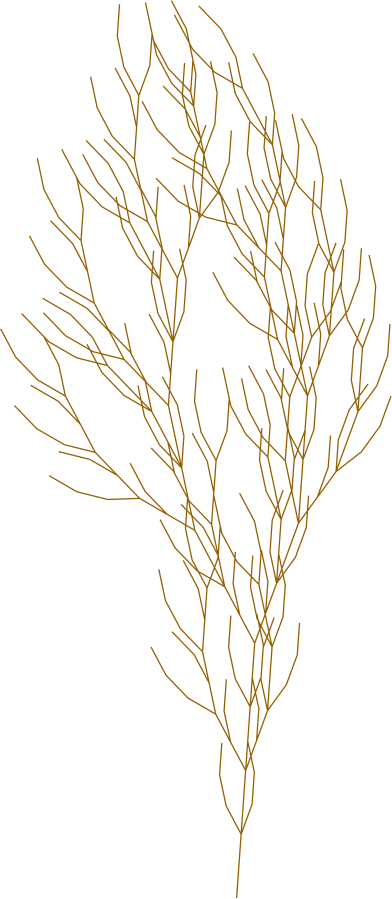
\includegraphics[height=7cm]{L-system-fractal.svg.png}
	\caption{Przykład stworzonej struktury za pomocą L-systemu}
    \label{fig:lsystreeexample}
\end{figure}

\section{Struktura L systemu}


L-systemy są obecnie powszechnie nazywane parametrycznymi L-systemami, definiowanymi jako krotka:

\begin{gather}
	G = (V, \omega, P),
\end{gather}
gdzie

\begin{itemize}
	\item[-] V (alfabet) -- to zbiór symboli zawierający zarówno elementy, które można zastąpić (zmienne), jak i te, których nie można zastąpić ("stałe" lub "terminale")
	\item[-] \(\omega\) (początek, aksjomat lub inicjator) -- to ciąg symboli z V, który określa stan początkowy systemu.
	\item[-] P  -- to zbiór reguł produkcji lub produktów określających sposób zastępowania zmiennych przez kombinacje stałych i innych zmiennych. Produkcja składa się z dwóch ciągów: poprzednika i następnika. Dla każdego symbolu A, który jest członkiem zbioru V i nie występuje po lewej stronie żadnego iloczynu w P, zakłada się tożsamość iloczynu A → A; symbole te nazywamy stałymi lub terminalnymi.
	% \item \textbf{-------------}
	% \item[-] Alfabet jest zbiorem skończonym, a jego elementami są symbole. Natura symboli nie jest istotna, ich jedyną funkcją jest odróżnianie od siebie nawzajem. Ciąg znaków w alfabecie to skończony ciąg znaków w alfabecie. W naszych zadaniach alfabet będzie się składał z najzwyklejszych znaków, a ciągi nad alfabetem będą najzwyklejszymi ciągami.
	% \item[-] Aksjomat to pewien ciąg znaków w alfabecie.
	% \item[-] Każda reguła jest parą składającą się z poprzednika i następnika. Poprzednik to znak z alfabetu, a następnik to łańcuch nad alfabetem. Oto przykład takiej pary: A \(\rightarrow\) FBFA+HFA+FB-FA (strzałka oddziela poprzednika od następnika). Znaki poprzedzające muszą być unikalne na liście reguł.
\end{itemize}

W standardowej wersji L-systemów reguły wnioskowania są następujące:
\begin{gather}
	v \rightarrow \omega,
\end{gather}
gdzie $v$ jest znakiem danego alfabetu $V$, $\omega \in V^* $ jest łańcuchem
znaki (ewentualnie puste) w tym samym alfabecie.
Każdą regułę można więc interpretować jako
podział komórki $(|\omega| > 1)$, lub jej modyfikację $(|\omega| = 1)$, lub
jako jej śmierć $(|\omega| = 0)$.

Na tabeli \ref{tab:table1} przedstawiono przykład L-systemu.
\begin{table}[h]
	\caption{Przykład stworzonej struktury za pomocą L-systemu}
	\label{tab:table1}
	\begin{center}
		\begin{tabular}{|c|c|l|}
			\hline
			Alfabet & Aksjomat & Reguły \\ [0.5ex]
			\hline
			\{ \crnrs{A}, \crnrs{B}, \crnrs{F}, \crnrs{H},\crnrs{J},\crnrs{+}, \crnrs{-} \} &
			\crnrs{FB}                            &
			\crnrs{A} $\rightarrow$ \crnrs{FBFA+HFA+FB-FA} \\
			& & \crnrs{B} \(\rightarrow\) \crnrs{FB+FA-FB-JFBFA} \\
			& & \crnrs{F} \(\rightarrow\) \crnrs{} \\
			& & \crnrs{H} \(\rightarrow\) \crnrs{-} \\
			& & \crnrs{J} \(\rightarrow\) \crnrs{+}                                            \\
			\hline
		\end{tabular}
	\end{center}
\end{table}

Po zdefiniowaniu L-systemu, zaczyna ona ewoluować zgodnie ze swoimi zasadami. 
Stanem początkowym L-systemu jest jego aksjomat. 
Wraz z dalszym rozwojem ta linia opisująca stan ulegnie zmianie. 
Rozwój L-systemu odbywa się cyklicznie. W każdym cyklu rozwoju ciąg 
jest oglądany od początku do końca, symbol po symbolu. 
Dla każdego znaku wyszukiwana jest reguła, dla której ten znak 
jest poprzednikiem. Jeśli taka reguła nie zostanie znaleziona,
znak jest pozostawiony bez zmian. Innymi słowy, dla tych znaków \crnrs{X},
dla których nie istnieje reguła jawna, obowiązuje reguła domyślna: \crnrs{X} $\rightarrow$ \crnrs{X}.
Jeśli zostanie znaleziona pasująca reguła, znak poprzednika jest
zastępowany przez łańcuch następnika z tej reguły.

Dla ilustracji rozważmy następujący L-system
(nazywamy go glon (łat. \textit{Algæ}), ponieważ jego rozwój
 modeluje wzrost pewnego gatunku alg) w tabeli \ref{tab:table2}:

\begin{table}[h]
	\caption{Przykład stworzonej struktury za pomocą L-systemu}
	\label{tab:table2}
	\begin{center}
		\begin{tabular}{|c|c|l|}
			\hline
			Aksjomat & Reguły \\ [0.5ex]
			\hline
			\crnrs{A} & 
			\crnrs{A} $\rightarrow$ \crnrs{B} \\

			& \crnrs{B} $\rightarrow$ \crnrs{AB} \\
			\hline
		\end{tabular}
	\end{center}
\end{table}

W tabeli \ref{tab:table3} przedstawiono stany tego L-systemu
odpowiadające pierwszym dziesięciu cyklom rozwoju systemu.

\begin{table}[h]
	\caption{Przykład stworzonej struktury za pomocą L-systemu}
	\label{tab:table3}
	\begin{center}
		\begin{tabular}{|c|l|}
			\hline
			Generacja & Stan \\ [0.5ex]
			\hline
			0 & \crnrs{A} \\
			1 & \crnrs{B} \\
			2 & \crnrs{AB} \\
			3 & \crnrs{BAB} \\
			4 & \crnrs{ABBAB} \\
			5 & \crnrs{BABABBAB} \\
			6 & \crnrs{ABBABBABABBAB} \\
			7 & \crnrs{BABABBABABBABBABABBAB} \\
			8 & \crnrs{ABBABBABABBABBABABBABABBABBABABBAB} \\
			\hline
		\end{tabular}
	\end{center}
\end{table}

Można zauważyć, że długości ciągów kodujących stan takiego L-systemu tworzą ciąg liczb Fibonacciego,
czyli ciąg liczbowy, w którym każda liczba jest równa sumie dwóch
poprzednich. Ciągami Fibonacciego będą także numery znaków A i B
w tych ciągach. Bardziej zaskakujący jest fakt, że ciąg ciągów ma
taką samą prawidłowość jak ciąg liczb Fibonacciego: każdy ciąg jest sumą
(konkatenacją) dwóch poprzednich.

\section{Interpretacja ciągu znaków}

W celu dalszej graficznej interpretacji otrzymanych ciągów
należy wprowadzić pojęcie grafiki żółwia. Grafika żółwia
to zasada organizacji graficznej biblioteki wyjściowej oparta 
na metaforze żółwia, wyimaginowanego 
(a w niektórych eksperymentach rzeczywistego) urządzenia 
przypominającego robota, które porusza się po ekranie 
lub papierze i obraca w zadanym kierunku, 
pozostawiając za sobą (lub opcjonalnie nie pozostawiając) 
narysowaną linię o zadanym kolorze i szerokości.

Interpretacja znaków polega na zdefiniowaniu operacji dla symboli
(nie jest konieczne dla wszystkich) w alfabecie. Czynności, podobnie 
jak symbole, są z kolei definiowane
przez autora systemu. Rysunek ref przedstawia przykład interpretacji
symbolu (z kątem $\alpha$ równym 90 stopni) w następujący sposób:

\begin{itemize}
	\item[--] \crnrs{F} oznacza przejście do przodu i narysuj linię
	\item[--] \crnrs{-} oznaca obrót w kierunku przeciwnym do ruchu wskazówek zegara na kąt o mierze $\alpha^\circ$
	\item[--] \crnrs{+} oznaca obrót zgodnie z ruchem wskazówek zegara o $\alpha^\circ$ 
\end{itemize}

\begin{figure}[h]
	\begin{center}
		\begin{tikzpicture}
			\draw [ultra thick, ->] (3,0) -- (3,3);
			\draw [thick, dashed, ->] (3,0) -- (0,0);
			\draw [thick, dashed, ->] (3,0) -- (6,0);
			\draw [thick, dotted, ->] (3,1.5) to [out=180, in=90] (1.5,0);
			\draw [thick, dotted, ->] (3,1.5) to [out=0, in=90] (4.5,0);
			\draw [fill] (3,0) circle [radius=0.1];
			\node [above] at (2.5,0.5) {-$\alpha$};
			\node [above] at (3.5,0.5) {$\alpha$};
			\node [below] at (1.5, 2.5) {\textbf{\crnrs{-}}};
			\node [below] at (4.5, 2.5) {\textbf{\crnrs{+}}};
			\node [above] at (3,3) {\textbf{\crnrs{F}}};
			\node [left] at (0,0) {\textbf{\crnrs{-F}}};
			\node [right] at (6,0) {\textbf{\crnrs{+F}}};
			\node [below] at (3,-0.1) {\textbf{$O$}};
		\end{tikzpicture}
	\end{center}
	\caption{Przykładowa interpretacja symboli}
	\label{fig:interpret}
\end{figure}

\section{L-systemy i modelowanie procesów wzrostu}

\chapter{Implementacja} 

\section{Wykorzystane narzędzia}

\subsection{Język i środowisko}

\subsection{Biblioteka Proctree}

\subsection{Biblioteka nlohmann Json}

\subsection{OpenGL}

\section{Funkcjonalność aplikacji}

\subsection{Planowanie drzew}

\subsection{Symulacja wzrostu}

\subsection{Ustawianie parametrów}

\subsection{Ustawianie tekstur}

\subsection{Zapis do pliku}

\section{Struktura programu}

\chapter{Testy i rezultaty}

\section{Wydajność}
\section{Porównanie z innymi rozwiązaniami}

\chapter{Podsumowanie}


\bibliographystyle{ieeetr}
\bibliography{bibliography/bib}
\addcontentsline{toc}{chapter}{Bibliografia}

\end{document}